\chapter{数值实验}
让观测站在 $X$ 轴上运动,观测站的加速度矢量为
 $a = [0.01,0,0]^T$,初始速度为0,初始位置为 $B_0 = (5km,0,0)$,在 $(x_0,y_0,z_0) \in [0,1000]\times[0,1000]\times[0,1000]$,$(v_x,v_y,v_z) \in [0,10]\times[0,10]\times[0,10]$的范围随机选取100,做100 Monte Carlo实验,并取 $\sigma = 0.0001rad$
\begin{figure}[htbp]
	\vspace{13pt}
	\centering
	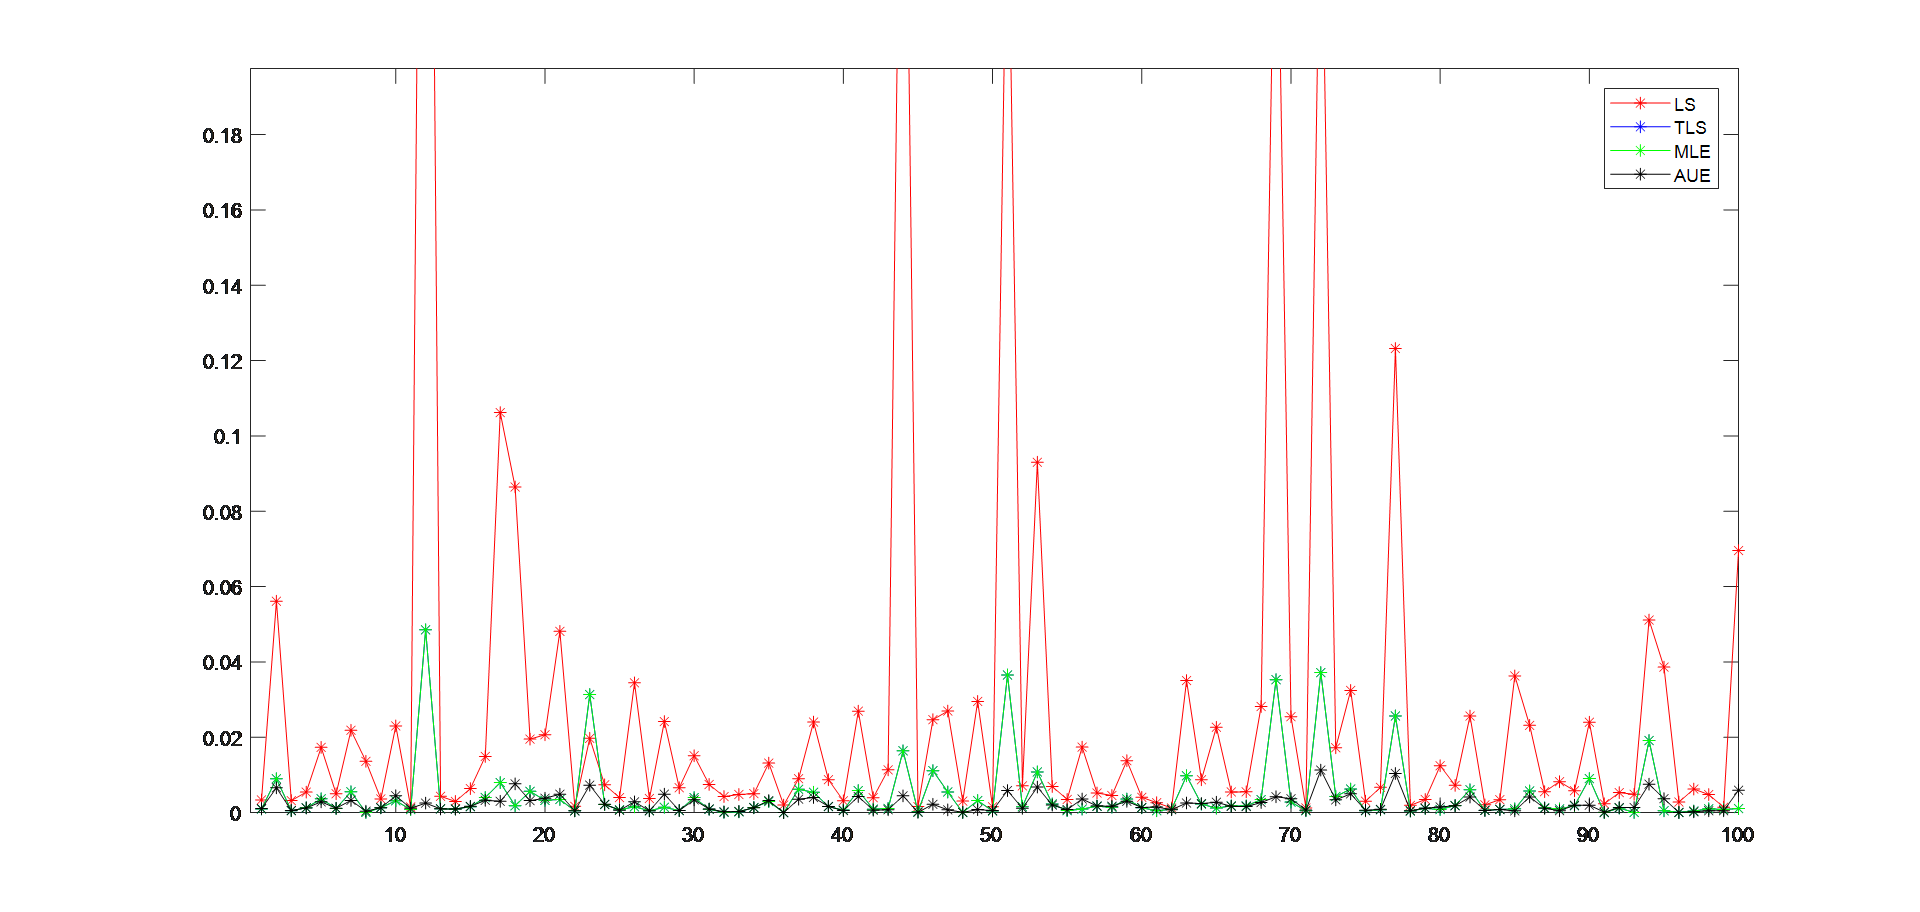
\includegraphics[scale=0.5]{images/100MonteCarlo.png}
	\caption{100次Monte Carlo实验算法距离相对误差图}
\end{figure}

根据上图可以看出,在100次Monte Carlo实验中,对目标的初始状态 $\bm{X}_0$求解结果的相对误差进行比较。AUE算法的结果相对较好,且最为稳定,而OLS算法的结果在多数情况下表现得较好,但是并不稳定,有时会产生较大的误差。TLS算法以及使用TLS求解估计值做为初值的MLE算法的结果相对OLS较好,且比OLS稳定,但比AUE算法的结果较差。
\begin{figure}[htbp]
	\vspace{13pt}
	\centering
	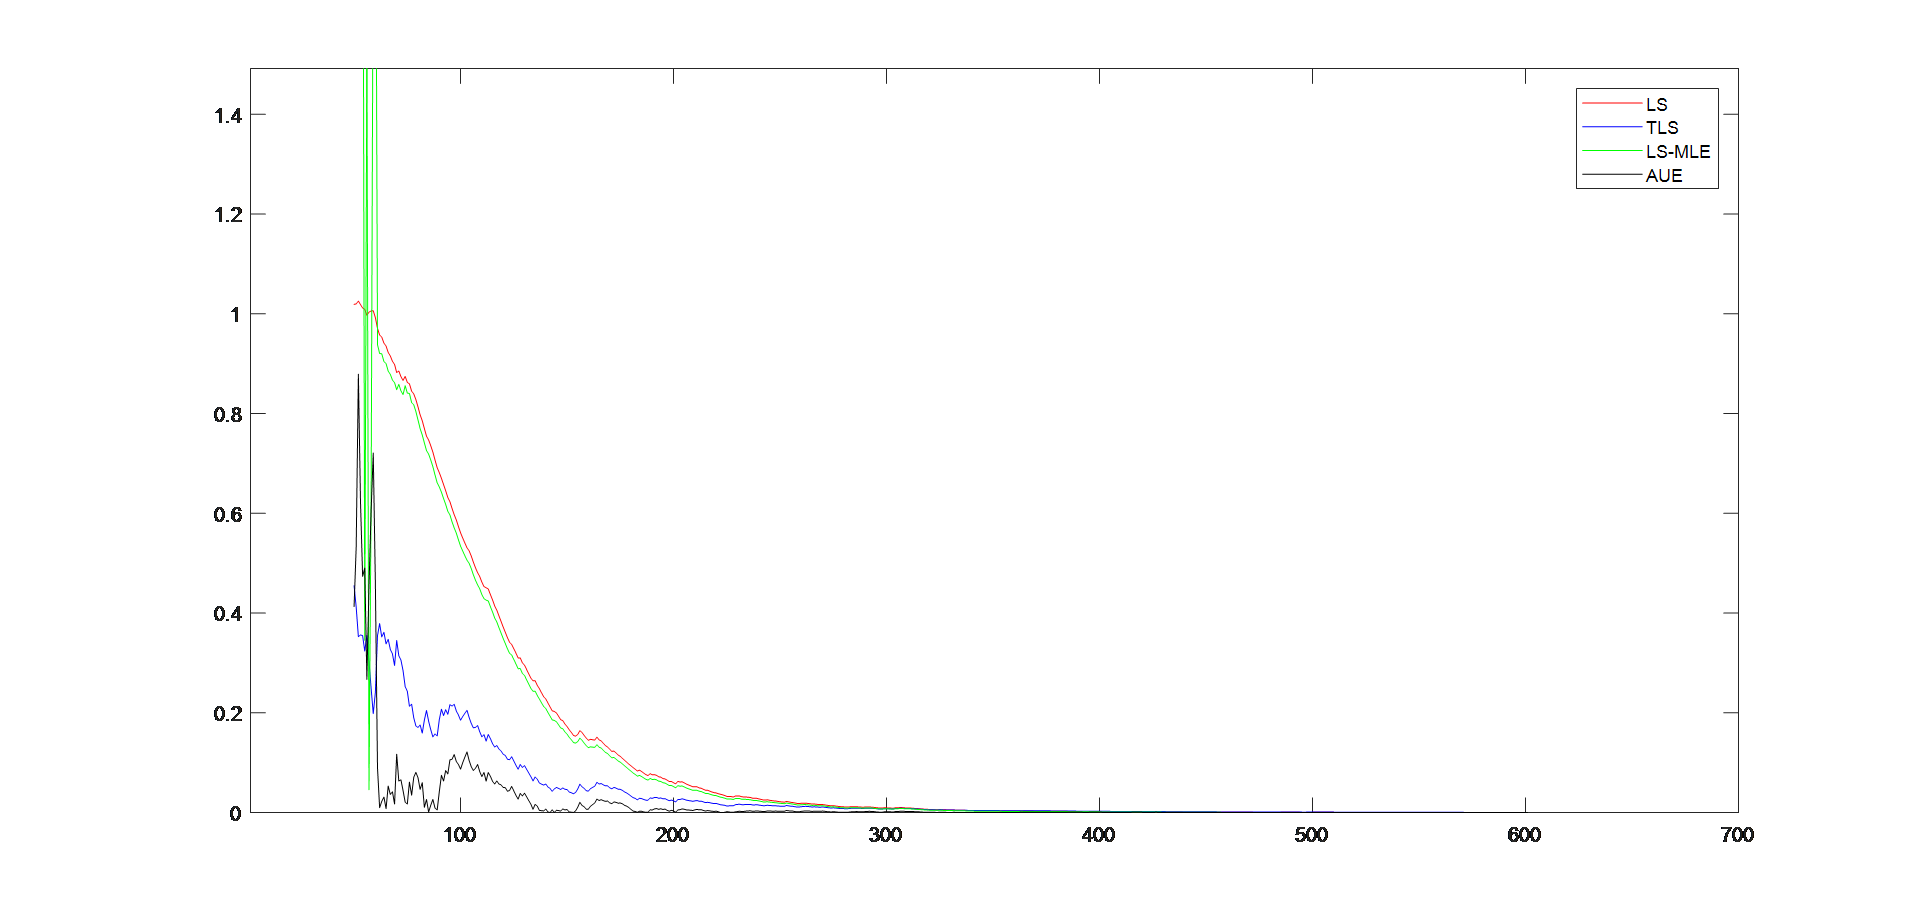
\includegraphics[scale=0.5]{images/singleline.png}
	\caption{前k个时间段求解的距离相对误差图}
\end{figure}